%%%%%%%%%%%%%%%%%%%%%%%%%%%%%%%%%%%%%%%%%%%%%%%%%%%%%%%%%%%
% --------------------------------------------------------
% Rho
% LaTeX Template
% Version 2.1.1 (01/09/2024)
%
% Authors: 
% Guillermo Jimenez (memo.notess1@gmail.com)
% Eduardo Gracidas (eduardo.gracidas29@gmail.com)
% 
% License:
% Creative Commons CC BY 4.0
% --------------------------------------------------------
%%%%%%%%%%%%%%%%%%%%%%%%%%%%%%%%%%%%%%%%%%%%%%%%%%%%%%%%%%%

\documentclass[9pt,a4paper,twoside]{rho-class/rho}
\usepackage[english]{babel}

%% Spanish babel recomendation
% \usepackage[spanish,es-nodecimaldot,es-noindentfirst]{babel}

\setbool{rho-abstract}{true} % Set false to hide the abstract
\setbool{corres-info}{true} % Set false to hide the corresponding author section

%----------------------------------------------------------
% TITLE
%----------------------------------------------------------

%\journalname{Molecular Ecology}
\title{Genomic Evidence for Altitude-Driven Adaptive Divergence in a Color-Polymorphic Montane Insect}

%----------------------------------------------------------
% AUTHORS AND AFFILIATIONS
%----------------------------------------------------------

\author{}

%----------------------------------------------------------

\affil{}

%----------------------------------------------------------
% DATES
%----------------------------------------------------------

\dates{This manuscript was compiled on May 27, 2025}

%----------------------------------------------------------
% FOOTER INFORMATION
%----------------------------------------------------------

\leadauthor{}
\smalltitle{Altitude-Driven Adaptive Divergence}

%----------------------------------------------------------
% ARTICLE INFORMATION
%----------------------------------------------------------

\corres{}
\email{}

%----------------------------------------------------------
% ABSTRACT
%----------------------------------------------------------

\begin{abstract}
    Understanding how environmental gradients shape genetic and phenotypic variation is fundamental to evolutionary genetics. In this study, we investigate local adaptation in a montane insect species exhibiting striking color polymorphism along a steep altitudinal gradient (450–2,300 m) in the Fırtına Valley of Türkiye. Using genome-wide RAD-seq data from 71 individuals, we identified 92,048 polymorphic loci, including 1,113 putatively adaptive SNPs. Despite low genome-wide differentiation ($F_{ST} < 0.05$), \textcolor{red}{}adaptive loci showed elevated divergence, suggesting selection-driven structuring. Genome-wide association analyses revealed 101 SNPs significantly correlated with altitude, with bidirectional allele frequency shifts consistent with local adaptation. Discriminant analysis further identified three major-effect loci distinguishing color morphs, all of which were also significantly associated with elevation. These results highlight the interplay between selection, gene flow, and environmental heterogeneity in shaping genomic variation across elevation. Our findings provide insights into the genetic basis of phenotypic divergence and contribute to understanding how biodiversity is maintained under spatially variable selection pressures.
\end{abstract}

%----------------------------------------------------------

\keywords{Clinal variation, Local adaptation, Genotype–environment association, RAD sequencing, Adaptive divergence, Non-model insect}

%----------------------------------------------------------

\begin{document}
	
    \maketitle
    \thispagestyle{firststyle}
    % \tableofcontents
    \linenumbers

%----------------------------------------------------------

\section{Introduction}

    Understanding how environmental gradients shape genetic and phenotypic variation is a central question in evolutionary ecology. Altitudinal and latitudinal gradients, in particular, serve as powerful natural laboratories for examining the interplay between gene flow, selection, and drift across spatially variable environments (\cite{Wogan2018}; \cite{Kelly2019}). These gradients impose structured ecological variation—such as shifts in temperature, humidity, and oxygen availability—that can drive local adaptation by favoring different alleles or traits at different elevations (\cite{Muir2014}). By investigating how genomic and phenotypic diversity align with these gradients, researchers can uncover the evolutionary mechanisms that underlie population differentiation and adaptation (\cite{Merilä2014}; \cite{Waldvogel2020}).

    Altitudinal gradients are especially informative because they generate sharp environmental transitions over short geographic distances (\cite{Chown2003}; \cite{Flatt2016}), often enhancing both gene flow limitation and divergent selection. This can result in population isolation due to isolation by distance (IBD), while also imposing strong selective pressures—including temperature variation, hypoxia, and habitat structure—that shape genetic differentiation through local adaptation (\cite{Sexton2014}; \cite{Stankowski2017}; \cite{Bradburd2019}). Combined with tools like genotype–environment association (GEA) analyses, altitudinal clines have become a valuable framework for identifying genetic loci under spatially varying selection (\cite{Hancock2011}; \cite{Slatyer2014}; \cite{Pluess2016}). In many systems, clinal variation in traits or allele frequencies provides insight into how selection acts across heterogeneous landscapes (\cite{Mayekar2022}; \cite{Tyrmi2020}; \cite{Soliani2020}).

    One well-documented axis of altitudinal divergence is color polymorphism, especially in invertebrates. Color traits in insects are often involved in thermoregulation, camouflage, and ecological specialization, influencing both survival and fitness (\cite{Forsman2008}; \cite{Zeuss2014}; \cite{Kozlov2022}). Thermal melanism—the tendency for darker individuals to occur in colder, higher elevations—is a widely reported pattern, attributed to the thermal benefits of increased solar absorption (\cite{Clusella-Trullas2020}). However, deviations from this pattern in many ectothermic species suggest that additional ecological drivers such as habitat complexity and predation also influence color trait evolution (\cite{Karlsson2008}; \cite{Goodman2021}).

    Beyond thermoregulation, color polymorphism can expand niche breadth by allowing populations to occupy a range of environmental conditions. This promotes broader distribution, ecological resilience, and potentially reduces extinction risk under environmental change (\cite{Forsman2008}; \cite{Wennersten2009}; \cite{Kozlov2022}). Understanding the genetic basis of such variation is essential for linking phenotypic divergence to evolutionary processes and identifying the drivers of population persistence and speciation (\cite{Forsman2016}; \cite{McLean2014}).

    In this context, the montane bush cricket \textit{Isophya rizeensis} (Orthoptera: Tettigoniidae: Phaneropterinae: Barbitistini) offers an excellent system to study altitudinal adaptation (\cite{SEVGILI2003}). This univoltine, color-polymorphic species is endemic to the Fırtına Valley of the Pontic Mountains in northeastern Türkiye and occupies a broad elevational range from 300 to 2,200 meters. Males exhibit striking dorsal color polymorphism, with darker individuals occurring at lower elevations and paler morphs at higher altitudes  (\cite{Çağlar2014})—a pattern that contradicts predictions of thermal melanism which associates dark coloration with higher, cooler habitats (\cite{CLUSELLATRULLAS2007}).

    Physiological data suggest that darker individuals warm more quickly and reach higher body temperatures than paler ones, which could be maladaptive in subalpine habitats where surface temperatures regularly exceed 40°C due to intense solar radiation (\cite{Kuyucu2016}). In such environments, paler coloration may reduce overheating risk, offering a selective advantage in sparsely vegetated, high-altitude zones. Despite these observations, the genetic architecture underlying this color polymorphism—and its relationship with elevation and population differentiation—remains unknown. Moreover, it is unclear whether phenotypic divergence is maintained by selection or emerges from neutral processes like drift and limited gene flow.

    In this study, we test the hypothesis that altitude-driven selection maintains color polymorphism in \textit{I. rizeensis} by integrating genome-wide RAD sequencing with high-resolution population genetic and genotype–phenotype association analyses. Specifically, we aim to:

    \begin{enumerate}
    \item Characterize population structure and connectivity along an altitudinal gradient.
    \item Quantify neutral vs. adaptive genetic differentiation to disentangle drift from selection.
    \item Identify loci associated with altitude and color polymorphism, clarifying whether these patterns arise from a common genetic basis.
    \end{enumerate}

    By coupling genomic data with environmental and phenotypic gradients, our study sheds light on the mechanisms driving local adaptation and the maintenance of intraspecific diversity in heterogeneous montane ecosystems. We show that a small subset of adaptive loci can remain highly differentiated despite extensive gene flow across a narrow altitudinal gradient, providing mechanistic insight into how spatially varying selection maintains functional polymorphism. Our reference-free analytical framework is broadly applicable to non-model taxa, and our findings contribute to ongoing debates about the genomic architecture of local adaptation. More broadly, this work offers empirical grounding for forecasting the evolutionary resilience of montane biodiversity under accelerating environmental change.

\section{Materials and Methods}

    \subsection{Sample Collection and Sequencing}

        Male specimens used in this study were collected between June and August 2006 from 11 locations along an altitudinal gradient ranging from 450 to 2,300 meters above sea level in the Fırtına Valley (Figure 1) via sweep netting and categorized according to color as described in \cite{Çağlar2014}. DNA was extracted from the hind femora of individuals using the \textsc{E.Z.N.A.}® Insect DNA Kit (Omega Bio-Tek), following the manufacturer’s protocol. Genome-wide data were generated via Restriction site–Associated DNA sequencing (i.e., RAD sequencing). Paired-end RAD libraries were constructed using the \textit{PstI} restriction enzyme, following the protocol detailed in \cite{Ali2016}. Sequencing was conducted at an average depth of 10× on an Illumina HiSeq4000 at the UC Davis Genome Center. In total, we generated RAD sequencing data from 75 \textit{I. rizeensis} individuals along the Fırtına Valley, averaging 5–7 individuals per location/altitude.
    
    \subsection{Alignment and filtering}

        Due to the absence of a reference genome for \textit{I. rizeensis} or in a closely related species, we generated a de novo RAD sequence reference library following the custom procedure given in \cite{SağlamMolEcol2016} (for details see supplementary materials). Raw reads from each individual were aligned to the reference set of RAD-contigs using the \textsc{bwa-mem} algorithm (\cite{Li2010}; \cite{Li2013}). The resulting \textsc{sam} files were converted to coordinate-sorted \textsc{bam} files using \textsc{samtools} (\cite{Danecek2021}), and duplicate reads were marked with \textsc{Picard tools} (http://broadinstitute.github.io/picard). Paralog regions were identified using \textsc{ngsParalog} (https://github.com/tplinderoth/ngsParalog) and removed from subsequent analysis.

    \subsection{SNP discovery and genotyping}

        Polymorphic sites were identified using \textsc{angsd}  (\cite{Korneliussen2014}) by calculating genotype likelihoods (\texttt{-GL $1$}), major and minor alleles (\texttt{-doMajorMinor $1$}), minor allele frequencies (\texttt{-doMaf $1$}), and generating \textsc{BCF/VCF} files (\texttt{-doBcf $1$}). Polymorphic sites were filtered to include only those with a minor allele frequency (MAF) of $0.05$ or higher (\texttt{-minMaf 0.05}). Additional filtering parameters included a minimum base quality score of $20$ (\texttt{-minQ $20$}), a minimum mapping quality of $10$ (\texttt{-minMapQ $10$}), and a posterior genotype probability threshold of $0.85$ (\texttt{-postCutoff $0.85$}). Only properly paired reads ( \texttt{-only\_proper\_pairs $1$}) were considered, and sites were retained only if the probability of them being polymorphic was statistically significant (\textit{P} < $10^{-12}$). Finally we filtered out any site that had an average per individual read depth under $6X$ and was not present in at least $50\%$ of individuals in each population.

    \subsection{Population Genetic Structure}

        Population genetic structure was assessed using Principal Component Analysis (PCA). First, a genetic covariance matrix was calculated between individuals in \textsc{PCAngsd} (\cite{Meisner2018}) based on genotype likelihoods. The covariance matrix was then subjected to eigenvalue decomposition in R (\cite{R2024}, version 4.2.0) to extract the principal component axes summarizing genetic variation and the first two principal components (PCs) were visualized in R.
       
        Admixture analyses were conducted with \textsc{NgsAdmix} (\cite{Skotte2013}) to estimate individual ancestry proportions based on genotype likelihoods. Analyses were performed for K values ranging from 2-5, with 10 independent runs for each K value to account for stochastic variation and avoid convergence to local optima. The most likely number of clusters was identified using the $\Delta{K}$ method of \cite{Evanno2005}, which calculates the rate of change in log-likelihood values across successive K values and admixture proportions for each K value were visualized in R.

    \subsection{Genetic Differentiation and Isolation By Distance (IBD)}

        Genetic differentiation was assessed by calculating pairwise $F_{ST}$ values between sampling sites along the altitudinal gradient. Genome-wide $F_{ST}$ estimates were derived using \textsc{Angsd}, beginning with the calculation of the joint site frequency spectrum (2D-SFS) for each population pair. Global weighted $F_{ST}$ values were then computed with the \texttt{realSFS} module (\cite{Nielsen2012}). To evaluate patterns of isolation by distance (IBD), a Mantel test was performed to assess the correlation between geographic and genetic distances. A Euclidean distance matrix between populations was generated using the \textsc{Geographic Distance Matrix Generator} v1.2.3 (\Cite{Ersts2024}) and served as the predictor variable, while the linearized pairwise $F_{ST}$ matrix [$F_{ST}$/(1 - $F_{ST}$)] was used as the response variable. IBD patterns were analyzed through Pearson and Spearman correlation Mantel tests with 999 permutations, implemented in R using the \texttt{vegan package} (\cite{Oksanen2001}; \cite{Mantel1967}).
 
    \subsection{Comparing Neutral and Adaptive Genetic Variation}

        To identify putatively adaptive loci, we used the \texttt{pcadapt} function in \texttt{PCAngsd} (\cite{Meisner2018}), which detects outliers based on population structure (\cite{Luu2017}). Unlike $F_{ST}$ based outlier methods that identify loci based on genetic differentiation (\cite{antao2008}; \cite{whitlock2015}), \texttt{pcadapt} detects SNPs significantly associated with major axes of genetic variation, as captured by principal components (PCs). This method relies on the correlation between SNPs and PCs, eliminating the need for predefined population assignments or differentiation thresholds. As a result, it reduces biases introduced by demographic history and heterogeneous gene flow (\cite{Luu2017}).
        
        The analysis was conducted using the Mahalanobis distance statistic across principal components, with significance determined by a chi-square ($\chi^2$) distribution with $K$ degrees of freedom based on the number of significant PC axes after correcting for multiple testing. We identified one significant principal component ($K = 1$) based on Velicier’s minimum average partial (MAP) test (\cite{Shriner2011}). To mitigate inbreeding effects, SNPs deviating from Hardy-Weinberg equilibrium due to inbreeding were filtered using the \texttt{--inbreedSites} and \texttt{--inbreed} options in \texttt{PCAngsd}, yielding a final dataset of $82,976$ SNPs, resulting in a genome-wide significance threshold of $6.03 \times 10^{-7}$ ($\chi^2 = 24.903$, $df = 1$, $\alpha = 0.05$) for determining putatively adaptive loci.

        Genetic diversity was estimated separately for neutral and adaptive loci by computing pairwise nucleotide differences ($\theta_{\pi}$) based on the folded site frequency spectrum (SFS) since we did not have a suitable outgroup for determining ancestral states. Allele frequency likelihoods were first calculated in \texttt{ANGSD} (\texttt{-doSaf 1}), followed by maximum likelihood estimation of the SFS using \texttt{realSFS}. Genome-wide $\theta_{\pi}$ was obtained using the \texttt{thetaStat} module (\texttt{-do\_stat}) by averaging per-site values across all RAD loci.

        To assess genetic differentiation, pairwise $F_{ST}$ values were calculated, and isolation by distance was evaluated via Mantel tests, correlating geographic and genetic distances separately for neutral and adaptive loci.


    \subsection{Genetic Variation Associated with Altitude}
    
        To investigate genetic variation associated with altitude, a genome-wide association study (GWAS) was conducted using score statistics (\texttt{-doAsso $2$}) in \textsc{Angsd}. The score test applies a generalized linear model framework, with posterior genotype probabilities as the dependent variable and altitude (\texttt{-yQuant}) as the predictor variable, calculating likelihood scores for each SNP independently (\cite{Skotte2012}).

        Association mapping included the identification of polymorphic sites (\texttt{-SNP\_pval 1e-06}), inference of major and minor alleles (\texttt{-doMajorMinor $1$}), and estimation of allele frequencies (\texttt{-doMaf $1$}). Stringent filtering criteria were applied to exclude SNPs with a minor allele frequency below $5\%$ (\texttt{-minMaf $0.05$}) or fewer than ten observations per genotype class (homozygous major, heterozygous, and homozygous minor; \texttt{-minHigh $10$}). Likelihood ratio test (LRT) scores for each SNP were converted to \textit{P}-values, assuming a chi-square ($\chi^2$) distribution with one degree of freedom. A Bonferroni correction was applied to control for multiple testing.
        
        To examine allele frequency patterns at significantly associated sites, the frequency of the reference allele (defined as the minor allele across the entire dataset) was plotted against altitude. This analysis highlights altitude-driven genetic variation by illustrating changes in allele frequencies with elevation.

    \subsection{Genetic Discrimination of Color Morphs}
        To investigate genetic variation associated with color morphs, a Discriminant Analysis of Principal Components (DAPC) was performed using the R package \texttt{adegenet} (v2.1.1; \cite{Jombart2008}; \cite{Jombart2011}). Genotypes were called in \textsc{Angsd} (\texttt{-doGeno $4$}) and exported as \texttt{VCF/BCF} files (\texttt{-doBcf $1$}) using a uniform prior (\texttt{-doPost 2}) and a posterior probability cutoff of $85\%$ (\texttt{-postCutoff $0.85$}). The DAPC retained principal component axes explaining up to $80\%$ of the variance, with color morph (dark vs. pale) specified as the grouping variable.
        
        To identify SNPs contributing most strongly to discrimination between color morphs, variable contributions of SNPs to the linear discriminant functions were examined. These contributions were hierarchically clustered using the \texttt{Average} method in the \texttt{snpzip} function of \texttt{adegenet}, grouping loci into "outlier" and "non-outlier" categories.
        
        Genotypic variation at the identified outlier loci was further explored by categorizing individuals based on genotypes either as heterozygous, homozygous for the minor allele, or homozygous for the major allele. Genotype distributions were visualized as a heatmap generated with \texttt{ggplot2} (\cite{ggplot2}), illustrating differences in genotypic states between dark and pale morphs.

\section{Results}

    \subsection{Alignment Statistics and SNP Discovery}

        Using our de novo reference assembly strategy, we identified $224,187$ unique RAD-loci ranging from $250$ to $800$ bp, with an average length of $324$ bp. Raw read alignments to the de novo set of reference RAD-contigs achieved a mapping success rate of $73\%$ to $83\%$, averaging $77\%$, with a mean individual read depth of approximately $5-6X$. Detailed data on raw read counts, raw alignments, and alignments after removing PCR duplicates are provided in Supplementary Table S1. Based on alignment statistics, we excluded individuals with fewer than $1,000,000$ aligned reads after all filters, resulting in a final dataset of $71$ individuals from $11$ locations (Table 1). Across all collection sites, we identified $9,616$ polymorphic loci and $92,048$ high-confidence SNPs (\textit{P} < $10^{-12}$) with a minor allele frequency $>0.05$, a minimum per individual read dept of $6X$ and present in $\geq50\%$ of individuals per population.
        
\begin{table}[!h]
    \small
    \captionsetup[table]{labelsep=space, 
        justification=raggedright, singlelinecheck=off}
    \caption{Altitude, coordinates, color category and samples sizes of \textit{I. rizeensis} used in this study.}
    \label{tab:my-table}
    \scalebox{1.3}{
    \begin{tabular}{@{}lllll@{}}
    \toprule
    Altitude (m) & Latitude & Longitude & Color & N \\ \midrule
    450          & 40.9856  & 40.9646   & DARK  & 7 \\
    850          & 40.9406  & 40.9850   & DARK  & 6 \\
    900          & 40.9166  & 40.9456   & DARK  & 7 \\
    1000         & 40.9075  & 40.9479   & DARK  & 7 \\
    1100         & 40.8880  & 40.9297   & PALE  & 7 \\
    1200         & 40.8630  & 40.9342   & PALE  & 5 \\
    1300         & 40.8638  & 40.9501   & PALE  & 5 \\
    1900         & 40.8548  & 41.0125   & PALE  & 7 \\
    2000         & 40.7998  & 40.9217   & PALE  & 7 \\
    2100         & 40.7995  & 40.9588   & PALE  & 7 \\
    2300         & 40.7915  & 40.9574   & PALE  & 6 \\ \bottomrule
    \end{tabular}%
    }
\end{table}

    \subsection{Population Genetic Structure and Differentiation}

        Principal Component Analysis (PCA) identified two distinct genetic clusters along PC1, corresponding to individuals from lower (dark-colored) and higher (pale-colored) altitudes (Figure 2A). However, PC1 and PC2 accounted for only $3.82\%$ and $2.08\%$ of the total genetic variation, respectively, indicating limited overall genetic divergence. A transitional zone was observed along PC1, comprising individuals from intermediate altitudes (1100–1900 meters).
        
        Admixture analysis, consistent with the PCA, identified K=3 as the optimal number of clusters (Supplementary Figure S1 and S2). Low and high altitude populations showed minimal admixture, predominantly belonging to distinct genetic ancestries whereas mid-altitude populations (1100–1900 meters) formed a transition zone with mixed ancestry, corroborating PCA findings (Figure 2B). Along the altitudinal gradient, the proportion of low-altitude ancestry (black) decreased, while high-altitude ancestry (green) increased, reflecting a reciprocal relationship between genetic components and elevation (Figure 2B).

        Pairwise $F_{ST}$ comparisons revealed relatively low genetic differentiation along the altitudinal gradient and between populations (< $0.05$), indicating substantial genetic connectivity across the landscape (Supplementary Figure S3). Despite the overall low divergence a Mantel test revealed a significant relationship between linearized $F_{ST}$  [$F_{ST}/(1 - F_{ST})$] values and geographic distance for both Pearson (\textit{$r_p$} = $0.838$, \textit{P} = $0.001$) and Spearman (\textit{$r_s$} = $0.869$, \textit{P} = $0.001$) correlation tests, indicating a clear pattern of IBD (Figure 2C).

    \subsection{Comparing Neutral and Adaptive Variation}

        \textsc{PCAdapt} identified 1,113 putatively adaptive SNPs within 809 distinct RAD-loci and 81,863 neutral SNPs within 8,699 distinct RAD-loci. Genome-wide mean genetic diversity ($\theta_\pi$) was generally high across the altitudinal gradient, ranging from 0.058 to 0.065 (Figure 3A, Table S3). Mean genetic diversity values for neutral and adaptive loci were largely similar along the altitudinal gradient. However, we observed a slight increase in neutral genetic diversity relative to adaptive genetic diversity at mid-altitudes (excluding 1,000 meters), with significant differences in mean $\theta_\pi$ between 900 and 1,900 meters (Figure 3A, Table S3).
    
        To compare genetic divergence, separate Mantel tests assessed correlations between geographic distance and linearized $F_{ST}$ [$F_{ST}$/(1 - $F_{ST}$) for adaptive and neutral loci. Genetic divergence increased with geographic distance for both categories, but the relationship was significantly steeper for adaptive loci (\textit{$r_p$} = 0.91, \textit{$r_s$} = 0.91, \textit{$P$} = 0.001) compared to neutral loci (\textit{$r_p$} = 0.84, \textit{$r_s$} = $0.87$, \textit{$P$} = 0.001) (Figure 3B). These results indicate greater divergence and signs of allelic fixation in adaptive loci at altitudinal extremes compared to neutral loci, suggesting a stronger role for selection in driving genetic differentiation along the altitudinal gradient.

    \subsection{Association Mapping of Altitudinal Variation}

        Genome-wide association studies using altitude as a quantitative variable was based upon $53,901$ SNPs that passed all filters leading to a genome wide significance of $9.276\times10^{-7}$ ($\alpha = 0.05$; LRT > $24.07$). Based on this threshold we identified 101 SNPs within 75 unique RAD-loci significantly associated with genetic variation along the altitudinal gradient (Table S4). Out of the 75 unique RAD-loci 73 were classified as "putatively adaptive" in prior analysis (Table S4). Notably, allele frequency changes showed a bidirectional pattern, with some loci displaying increased minor allele frequencies at low altitudes, while others increased at high elevations (Figure 4, Table S4). These opposing frequency shifts suggest that selection is acting on different genetic variants across the gradient, potentially reflecting locally adapted alleles in lowland vs. highland populations.
        
    \subsection{Genetic Discrimination between Color Morphs}

        Discriminant analysis of principal components (DAPC) based on dark and pale color morphs clearly separated individuals into two groups along the first discriminant function (DF1), with a high posterior assignment probability (0.97; Figure 5A). Pale individuals were perfectly classified (posterior success = 1.0), while $92.6\%$ of dark individuals were correctly assigned, with only two misclassified as pale.
   
        DF1 loadings identified three major-effect loci that significantly contribute to genetic differentiation between color morphs (Figure 5B). These loci displayed bimodal genotype distributions, with pale individuals nearly fixed for the major allele and dark individuals predominantly heterozygous (Figure 5C). Notably, all three loci were classified as "putatively adaptive" and showed significant associations with altitude (Table S4), reinforcing the connection between color polymorphism, altitudinal variation and local adaptation.

\section{Discussion}

Environmental gradients provide a powerful lens through which to explore the mechanisms of adaptation and the genomic architecture underlying phenotypic divergence. By integrating genome-wide data with environmental and phenotypic variables, this study contributes to a growing body of work demonstrating how spatially variable selection can drive differentiation at key loci, even in the face of high gene flow. Our findings exemplify how steep altitudinal transitions can shape both neutral and adaptive genomic variation and maintain discrete phenotypes, offering broad insights into the evolutionary processes that structure biodiversity.

    \subsection{Adaptive Differentiation Surpasses Neutral Expectations in Spatially Structured Environments}

    In systems with spatial environmental heterogeneity, distinguishing between neutral and adaptive differentiation is crucial for understanding how selection counteracts gene flow. Our findings illustrate that even in landscapes with low genome-wide differentiation, subsets of loci under selection can display strong divergence, particularly across sharp altitudinal transitions. 

    Nucleotide diversity across the altitudinal gradient showed similar trends for both neutral and adaptive loci, with genome-wide mean values remaining relatively uniform across populations and only minor fluctuations along the gradient. The only notable pattern was a slight increase in neutral genetic diversity in mid-altitude populations, likely due to gene flow between high- and low-altitude populations—a well-documented phenomenon in transition zones (\cite{Byars2009}; \cite{Polato2017}; \cite{Cortázar-Chinarro2017}). 

    In our focal system, divergence at adaptive loci was steepest at altitudinal extremes, echoing similar patterns observed in montane amphibians, plants, and insects experiencing divergent selection at ecological boundaries (\cite{Byars2009}; \cite{Polato2017}; \cite{Cortázar-Chinarro2017}; \cite{Zancolli2019}). While genome-wide differentiation was low ($F_{ST} < 0.05$), adaptive loci exhibited significantly greater divergence. The stronger correlation between genetic divergence and geographic distance for adaptive loci, relative to neutral markers, supports a role for isolation by environment (IBE) alongside isolation by distance (IBD) (\cite{Raeymaekers2017}; \cite{Jiang2019}; \cite{Wagutu2022}; \cite{Wakamiya2023}).

    \subsection{Spatially Structured Selection Maintains Phenotypic Polymorphism Despite Gene Flow}

    A longstanding question in evolutionary biology is how discrete phenotypic polymorphisms are maintained across continuous environmental gradients. Theory and empirical work increasingly highlight the role of spatially structured selection in maintaining such polymorphisms despite ongoing gene flow.

    In the montane context examined here, color polymorphism is tightly linked to altitude-associated loci, with distinct genotype–phenotype associations observed at both ends of the elevational range. Bidirectional allele frequency shifts at these loci suggest divergent selection favoring alternate alleles in different habitats, consistent with local adaptation (\cite{White2021}; \cite{Wadgymar2022}). This echoes findings from other systems where spatial environmental structure maintains polymorphism despite gene flow (\cite{Tigano2016}; \cite{Zancolli2019}; \cite{Berdahl2015}, \cite{Forester2016}).

    \subsection{Converging Genetic and Phenotypic Clines Highlight Mechanisms of Adaptive Divergence}

    The co-occurrence of genotype–phenotype associations with environmental gradients is a powerful signal of adaptation. Our results support a scenario in which a small number of large-effect loci contribute to phenotypic divergence, consistent with theories of adaptation via few large-effect mutations in high-selection environments (e.g., \cite{Yeaman2011}).

    Discriminant analysis revealed strong genetic structure between color morphs, with three loci significantly contributing to morph differentiation. These loci displayed bimodal genotype distributions—nearly fixed in pale individuals and heterozygous in dark morphs—indicative of strong selection pressures (\cite{Prince2017}, \cite{Thompson2019}, \cite{PereiraMartins2022}). The overlap between these loci and altitude-associated markers reinforces their relevance in environmentally mediated selection, consistent with observations in other taxa (\cite{Villoutreix2023}; \cite{Mullen2008}; \cite{Wittkopp2003}).

    Although the exact ecological drivers of coloration remain unresolved, hypotheses include thermoregulatory function, crypsis, or pleiotropic effects. Similar to \textit{Drosophila}, where pigmentation is regulated by dopamine and melanin pathways (\cite{Wright1987}; \cite{Wittkopp2003}), other systems also show diverse genetic mechanisms (\cite{MICHIE2010}; \cite{Bastide2016}). Our findings reflect the broader complexity of genotype–phenotype–environment interactions.

    \subsection{Limitations and Future Directions}

    As with many studies in non-model organisms, our inferences are constrained by the absence of a reference genome, limiting functional interpretation of adaptive loci. However, this challenge is shared across much of ecological genomics and highlights the value of RAD-seq–based frameworks in identifying candidate regions for future study.

    Our results are based on allele frequency patterns and genotype–environment associations rather than direct measures of fitness or functional assays. To strengthen inference, future work should integrate transcriptomic profiling, expression analyses, and functional tests (e.g., reciprocal transplant or common garden experiments). Prior studies have emphasized the utility of such approaches for confirming the adaptive significance of genomic outliers (\cite{hoban2016finding}; \cite{fumagalli2013assessing}; \cite{lotterhos2019effect}). Despite these gaps, this system provides a valuable platform for exploring how environmental gradients drive adaptive genetic divergence.

    \section{Conclusion}

    Environmental gradients such as altitude offer natural laboratories for studying selection, gene flow, and phenotypic divergence. Our results demonstrate that even across short geographic distances, spatially variable selection can maintain strong genetic and phenotypic differentiation at a small number of loci. These findings contribute to broader questions about the persistence of functional polymorphisms under gene flow, the role of ecological boundaries in driving divergence, and the genomic architecture of local adaptation. As montane ecosystems face increasing environmental pressures, such insights are critical for forecasting the evolutionary resilience of highland biota and informing biodiversity conservation in a changing world.











\printbibliography
\clearpage\section{Figures}
\begin{figure}[h]
\centering
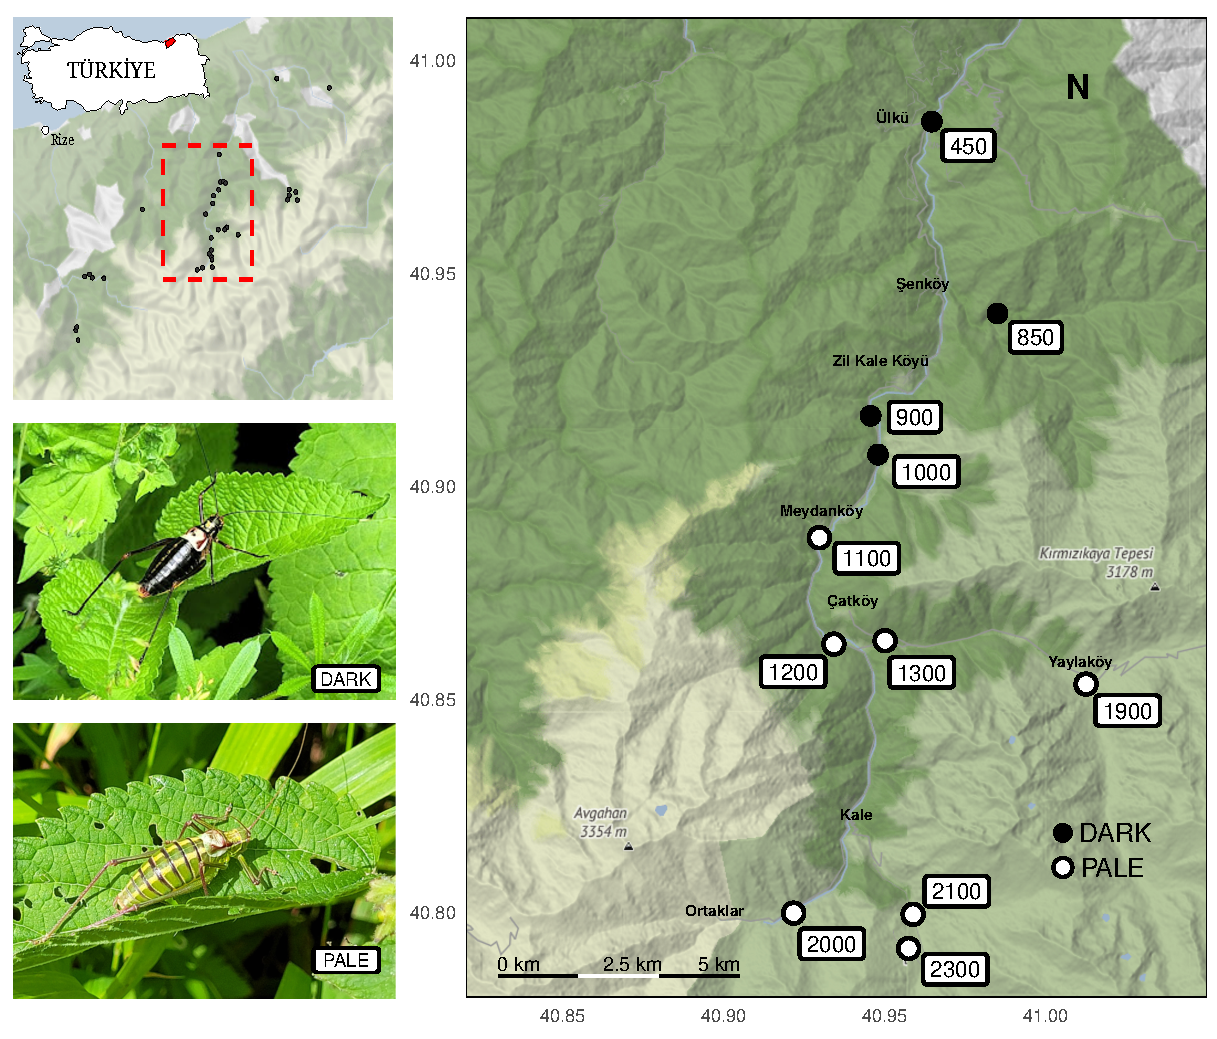
\includegraphics[width=1.8\columnwidth]{Figure_1.pdf}
\caption{Sampling locations of \textit{I. rizeensis} in the Fırtına Valley, Türkiye. Map showing the 11 collection sites along an altitudinal gradient within the Fırtına Valley. Village names and elevation values (in meters) are indicated. Sampling locations are categorized based on the two major color morphs of \textit{I. rizeensis} dark and pale.}
\label{Figure 1}
\end{figure}

\clearpage
\newpage
\begin{figure}[h]
\centering
\includegraphics[width=1.8\columnwidth]{Figure_2_v1.pdf}
\caption{Genetic structure and differentiation of \textit{I. rizeensis} along an alitudinal gradient in the Fırtına Valley. \textbf{(A)} Principal Component Analysis (PCA) of genetic variation, showing genetic structuring between lower-altitude (dark-colored) and higher-altitude (pale-colored) individuals along PC1. \textbf{(B)} Admixture proportions for $K=3$, illustrating distinct genetic ancestries at low (black) and high (green) altitudes, with mid-altitude populations exhibiting mixed ancestry. \textbf{(C)} Isolation-by-distance (IBD) pattern revealed by Mantel tests, showing significant patterns of genetic differentiation along the altitudinal gradient as measured by $F_{ST}$}
\label{Figure 2}
\end{figure}

\clearpage
\newpage
\begin{figure}[h!]
\centering
\includegraphics[width=0.8\columnwidth]{Figure_3.pdf}
\captionsetup[table]{labelsep=space, 
        justification=raggedright, singlelinecheck=off}
    \caption{Nucleotide diversity (A) and genetic differentiation (B) for adaptive and neutral loci in \textit{I. rizeensis} along an alitudinal gradient in the Fırtına Valley}
\label{Figure 3}
\end{figure}
\newpage
\begin{figure}[h!]
\centering
\includegraphics[width=0.8\columnwidth]{Figure_4_v1.pdf}
\caption{Altitudinal variation in allele frequencies for the 102 SNPs significantly associated with elevation in \textit{I. rizeensis}, showing two distinct trends where the minor allele frequency either increases or decreases with altitude.}
\label{Figure 4}
\end{figure}

\begin{figure*}[b!]
\centering
\includegraphics[width=1.8\columnwidth]{Figure_5.pdf}
\caption{Genetic differentiation between dark and pale color morphs of \textit{I. rizeensis} based on Discriminant Analysis of Principal Components (DAPC). (A) DAPC density plot along Discriminant Function 1 (DF1), showing clear separation between the morphs. (B) SNP loadings on DF1 identifying three major-effect loci contributing to morph differentiation. (C) Genotypic states at the three major loci along the altitudinal gradient. HMJ = Homozygote Major; HT = Heterozygote; HMN = Homozygote Minor}
\label{Figure 5}
\end{figure*}

\end{document}